%\documentclass[showpacs,preprintnumbers,amsmath,amssymb,superscriptaddress,aip]{revtex4-1}
\documentclass[twocolumn,showkeys,superscriptaddress]{revtex4}
\usepackage{graphicx}
%\usepackage{authblk}
%\usepackage{amssymb}
%\setlength{\parindent}{0in}

% General Latex  --------------------------------------------------
\def\beq{\begin{equation}}
\def\eeq{\end{equation}}
\def\beqar{\begin{eqnarray}}
\def\eeqar{\end{eqnarray}}
\def\nn{\nonumber}
\def\ol{\overline}
\def\para{\parallel}

% Operators  ------------------------------------------------------
\newcommand{\diff}[2]{\frac{d#1}{d#2}}
\newcommand{\diffs}[2]{\frac{d^2#1}{d#2^2}}
\newcommand{\pdiff}[2]{\frac{\partial#1}{\partial#2}}
\newcommand{\pdiffs}[2]{\frac{\partial^2#1}{\partial#2^2}}
\newcommand{\pdiffxy}[3]{\frac{\partial^2#1}{\partial#2 \partial#3}}
\newcommand{\pdt}{\partial_t}
\newcommand{\pdr}{\partial_r}
\newcommand{\pdth}{\partial_\theta}
\newcommand{\pdrr}{\partial^2_r}

\newcommand{\enum}[2]{{#1}\times10^{#2}} % 4.2x10^{3} = \enum{4.2}{3}

\newcommand{\vect}[1]{{\bf #1}}
%\newcommand{\vect}{\overrightarrow}
%\newcommand{\vect}{\vec}
\def\div{\nabla\cdot}
\def\grad{\nabla}
\def\curl{\nabla\times}
\newcommand{\gradpar}{\grad_\parallel}
\newcommand{\gradperp}{\grad_\perp}
\newcommand{\gradr}{\grad_r}
\newcommand{\defeq}{\ensuremath{\stackrel{\text{\tiny def}}{=}}}

\newcommand{\savg}[1]{\left<{#1}\right>}
\newcommand{\vavg}[1]{\left<{#1}\right>_V}
\newcommand{\thavg}[1]{\left<{#1}\right>_\theta}

% Variable names  -------------------------------------------------
\newcommand{\vpar} {v_\parallel}
\newcommand{\Apar} {A_\parallel}
\newcommand{\jpar} {j_\parallel}
\newcommand{\kpar} {k_\parallel}
\newcommand{\kperp} {k_\perp }
\newcommand{\vperp} {v_\perp }
\newcommand{\kthe}{k_\theta}

\newcommand{\Evec}{\ensuremath{\boldsymbol{{\rm E}}}}
\newcommand{\Bvec}{\ensuremath{\boldsymbol{{\rm B}}}}
\newcommand{\Jvec}{\ensuremath{\boldsymbol{{\rm J}}}}
\newcommand{\Fvec}{\ensuremath{\boldsymbol{{\rm F}}}}
\newcommand{\fvec}{\ensuremath{\boldsymbol{{\rm f}}}}
\newcommand{\vE}{\ensuremath{\boldsymbol{{\rm v}_{E}}}}
\newcommand{\bo}{\ensuremath{\boldsymbol{{\rm b}_0}}}
\newcommand{\bvec}{\ensuremath{\boldsymbol{{\rm b}}}}
\newcommand{\xvec}{\ensuremath{\boldsymbol{{\rm x}}}}
\newcommand{\yvec}{\ensuremath{\boldsymbol{{\rm y}}}}
\newcommand{\zvec}{\ensuremath{\boldsymbol{{\rm z}}}}
\newcommand{\vvec}{\ensuremath{\boldsymbol{{\rm v}}}}
\newcommand{\jvec}{\ensuremath{\boldsymbol{{\rm j}}}}

\newcommand{\bxgp}{\bvec\times\gradperp}

\newcommand{\vve}{\ensuremath{\boldsymbol{{\rm v}}_{e}}}
\newcommand{\vvi}{\ensuremath{\boldsymbol{{\rm v}}_{i}}}
\newcommand{\vpe}{v_{\parallel e}}
\newcommand{\vpi}{v_{\parallel i}}
\newcommand{\vvE}{\ensuremath{\boldsymbol{{\rm v}}_{E}}}
\newcommand{\vvD}{\ensuremath{\boldsymbol{{\rm v}}_{D}}}

\newcommand{\nuei}{\nu_{ei}}
\newcommand{\nuii}{\nu_{ii}}
\newcommand{\nue}{\nu_{e}}
\newcommand{\nuen}{\nu_{en}}
\newcommand{\nuin}{\nu_{in}}
\newcommand{\kpe}{\kappa_{\parallel e}}

\newcommand{\rs}{\rho_{s}}
\newcommand{\ri}{\rho_{i}}
\newcommand{\wci}{\Omega_{i}}
\newcommand{\wcix}{\Omega_{ix}}
\newcommand{\wce}{\Omega_{e}}
\newcommand{\tomega}{\tilde\omega}
\newcommand{\Isat}{I_{\rm sat}}
\newcommand{\fmie}{\frac{m_i}{m_e}}
\newcommand{\fmei}{\frac{m_e}{m_i}}


% Often used dimensions
\newcommand{\cm}{\rm cm}
\newcommand{\mm}{\rm mm}
\newcommand{\cmn}{{\rm cm}^{-3}}
\newcommand{\mn}{{\rm m}^{-3}}
\newcommand{\eV}{\rm eV}
\newcommand{\G}{\rm G}
\newcommand{\T}{\rm T}



\begin{document}

\title{Non-Modal Predictions of Turbulent Properties Applied to the Hasegawa-Wakatani Model}

\author{B. Friedman}
\email{friedman11@llnl.gov}

\affiliation{Department of Physics and Astronomy, University of California, Los Angeles, California 90095-1547, USA}
\affiliation{Lawrence Livermore National Laboratory, Livermore, California 94550, USA}


\author{T.A. Carter}

\affiliation{Department of Physics and Astronomy, University of California, Los Angeles, California 90095-1547, USA}



\begin{abstract}
Linear eigenmode analysis often fails to describe turbulence in model
systems that have non-normal linear operators, and thus
nonorthogonal eigenmodes, which can cause fluctuations to transiently grow faster than expected from eigenmode analysis. When combined with energetically conservative nonlinear mode mixing, 
transient growth can lead to sustained turbulence even in the absence of eigenmode instability. 
Since linear operators ultimately provide the turbulent fluctuations with energy, it is useful to define a growth rate that takes into account non-modal effects, allowing for
prediction of energy injection, transport levels, and possibly even turbulent onset in the subcritical regime. 
We define such a non-modal growth rate using a relatively simple model
of the statistical effect that the nonlinearities have on cross-phases and amplitude ratios of the system state variables. 
In particular, we model the nonlinearities as delta-function-like, periodic forces that randomize the state variables once every eddy turnover time. Furthermore, we estimate the eddy turnover
time to be the inverse of the least stable eigenmode frequency or growth rate, which allows for prediction without nonlinear numerical simulation. We test this procedure on the 2D and 3D Hasegawa-Wakatani model
[A. Hasegawa and M. Wakatani, Phys. Rev. Lett. 50, 682 (1983)] as well as on a modified subcritical version of the 3D Hasegawa-Wakatani model and find that
the non-modal growth rate is a good predictor of energy injection rates in some regimes, though not yet in the subcritical regime.
\end{abstract}

\maketitle

\section{Introduction}

The calculation of linear instabilities through normal mode analysis, which solves for the eigenvalues and eigenvectors of a linearized dynamical system,
has successfully predicted the turbulent onset criterion for many plasma and fluid systems.
Nevertheless, it is well-known in the hydrodynamics community that normal mode analysis has failed to predict turbulent onset in many experiments -- those in which the
turbulence is called subcritical~\cite{drazin1981}. 
In subcritical systems, turbulence develops even though all linear eigenvectors are stable such that infinitesimal perturbations on the equilibrium state cannot grow exponentially. 
Nevertheless, finite amplitude perturbations still excite turbulence through nonlinear instabilities.
Subcritical turbulence is common in plasmas as well, and several instances have been studied in the literature~\cite{waltz1985,scott1990,nordman1993,biskamp1995,drake1995,itoh1996,camargo1998,krommes1999,camporeale2009,schekochihin2012,highcock2012}. 

Since the hydrodynamics community has long studied subcritical turbulence, it has much to offer in terms of understanding of the phenomenon. Most significantly,
in the early 1990s, several researchers attributed the failure of normal mode analysis in predicting subcritical turbulent onset to the non-normality of linear operators of
dynamical systems~\cite{gustavsson1991,butler1992,trefethen1993,reddy1993,henningson1994,schmid2007}. A non-normal operator has 
eigenvectors that are not orthogonal to one another. One consequence of eigenvector nonorthogonality is that even when all eigenvectors decay exponentially under linear evolution, 
superpositions of eigenvectors can grow, albeit transiently.
In other words, certain fluctuation structures can access free energy from background gradients even though normal mode fluctuations cannot.
When combined with nonlinear effects, this allows for sustained subcritical turbulence by a bootstrapping process.
Such behavior is obscured by traditional normal mode analysis, which only effectively describes the long time asymptotic behavior of fluctuations under  
action of the linear operator. Transient growth, which can dominate turbulent evolution, must be found through non-modal calculations.

Non-modal analysis generally employs tools such as pseudospectra and maximum growth curves, which have been used to successfully explain
why turbulence is subcritical in various instances~\cite{trefethen1993,camargo1998}. 
However, they have not been used to predict onset criteria in subcritical systems (e.g. the transition Reynold's number in pipe flows).
This paper outlines and illustrates a non-modal method to make quantitative predictions of turbulent properties including turbulent onset criteria. 
Our approach is to define a non-modal growth rate that is analogous to an eigenmode growth rate, but which takes into account transient growth effects. 

To accomplish this, we model the effect that the nonlinearities have on the complex ratio of the state variables. Our model is one in which the 
nonlinearities randomize the complex ratios on a characteristic nonlinear time scale.
We estimate the nonlinear time scale by a characteristic linear time scale, taking either the inverse linear eigenmode frequency or growth rate as the linear time scale.
Between the nonlinear randomization, the system evolves linearly, and we use this evolution to calculate the non-modal growth rate. This non-modal growth rate takes the place of the eigenmode growth, which can be used
to give energy injection rates, turbulent saturation levels, and the turbulent onset criteria.
That is, we argue that a finite positive non-modal growth rate
indicates that turbulence can exist given a sufficiently large perturbative kick.

The paper is organized as follows: in Section~\ref{sec_hw_model}, we specify our illustrative model, the 2D and 3D Hasegawa-Wakatani model,
that we use throughout the paper and describe its linear non-normal properties,  while in Section~\ref{sec_non_norm_turb}, we explore the effect of linear non-normality in the model on turbulence. 
In Section~\ref{sec_nm_procedure}, we cover the details of our procedure to calculate the non-modal growth rate and compare show it to growth rates derived directly from nonlinear numerical simulations. 
Finally, in Section~\ref{sec_subcrit_prediction}, we modify the 3D Hasegawa-Wakatani model to make it subcritical and show to what degree our non-modal technique predicts the critical gradient for the onset of turbulence.

\section{Non-Normality of the Hasegawa-Wakatani Model} 
\label{sec_hw_model}

In order to illustrate and test our non-modal technique, we use as an example the well-known and well-analyzed Hasegawa-Wakatani (HW) model~\cite{hasegawa1983}.
In this section, we analyze the linear normality of the model.
We consider both the original 2D and the extended 3D~\cite{biskamp1995} versions of the model in a straight, unsheared magnetic field. 
The HW model consists of two equations for the density $n$ and the electrostatic potential $\phi$. The 3D version of the model is

\beqar
\label{n_eq}
\pdiff{n}{t} = - {\mathbf v_E} \cdot \grad n - \kappa \pdiff{\phi}{y} + \xi \gradpar^2 (n - \phi) - D \gradperp^4 n, \\
\label{phi_eq}
\pdiff{\gradperp^2 \phi}{t} = - {\mathbf v_E} \cdot \grad (\gradperp^2 \phi) + \xi \gradpar^2 (n - \phi) - D \gradperp^6 \phi
\eeqar
The normalizations are $\phi \to e \phi/T_e, n \to n/n_0, \grad \to \rho_s \grad , x,y,z \to x,y,z/\rho_s, t \to \omega_{ci} t $, where $\rho_s$ is the ion sound gyroradius at the electron temperature and $\omega_{ci}$ is
the ion cyclotron frequency. Additionally, $\mathbf{v_E} = \mathbf{b} \times \grad \phi$, where $\mathbf{b}$ is the magnetic field direction, $\xi = 4 \pi \omega_{ce}/\nu_{ei}$, where $\omega_{ce}$ is the electron cyclotron
frequency and $\nu_{ei}$ is the electron-ion collision frequency,
and $\kappa = \rho_s/L_n$, where $L_n$ is the density scale length. The terms $D \gradperp^4 n$ and $D \gradperp^6 \phi$ are artificial hyper-diffusion and hyper-viscosity used to dissipate
energy on small scales. We set $D \to 10^{-5}$ except in Sec.~\ref{sec_subcrit_prediction} where we set it to $0.5$.
We associate the direction $\mathbf{b}$ as the $z$ direction. The direction perpendicular $\mathbf{b}$ that
points opposite the density gradient is defined as the $x$ direction, and the $y$ direction is taken perpendicular to both of these.

In the analysis and numerical simulations, which we perform with the BOUT++ code~\cite{dudson2009}, we use periodic boundary conditions in
the $y$ and $z$ directions with zero-value boundaries in the $x$ direction. We use a domain size of $64 \rho_s \times 64 \rho_s \times 320 \rho_s$.
For the 2D version of the model, we replace $-\xi \gradpar^2$ with a single parameter $\alpha$ (defined as $\alpha = 4 \pi k_z^2 \rho_s^2 \omega_{ce} /\nu_{ei})$, 
which is commonly known as the adiabaticity parameter~\cite{camargo1995,camargo1998}. Additionally we use a domain size of $50 \rho_s \times 50 \rho_s$.
In numerical simulations, the turbulence can be suppressed due to the build-up of $k_y=0$ density and potential structures~\cite{biskamp1995}. To prevent this, we subtract out the $k_y=0$
density and potential components, which is the equivalent of adding source terms to Eqs.~\ref{n_eq} and~\ref{phi_eq}~\cite{friedman2012b}.

The degree of non-normality of the linear operator in the HW model is largely a function of the adiabaticity parameter~\cite{camargo1998}, or in the 3D case, of $\xi \gradpar^2$. 
A normal matrix is on that commutes with its adjoint: $\mathbf{D} \mathbf{D}^\dagger = \mathbf{D}^\dagger \mathbf{D}$.
The HW model has a normal linear operator in the adiabatic limit: $\alpha, \xi \to \infty$. 
This is evident when we transform the linear operator into a linear matrix by using a Fourier decomposition. Because we use a zero-value boundary condition in the $x$ direction, the
Fourier decomposition takes the form:

\beq
\label{fourier_form}
f_k = \int_0^{L_x,L_y,L_z} f(\mathbf{r}) \ {\rm sin} \left( k_x x \right) e^{i k_y y + i k_z z} d\mathbf{r}
\eeq
where $k_x = \pi l/L_x, k_y = 2 \pi m/L_y, {\rm and } \ k_z = 2 \pi n/L_z$ with $l, m, {\rm and } \ n$ integers.
The result for the 3D model is an equation for each mode $k = (k_x,k_y,k_z)$:

\beqar
\label{fourier_eqn}
\frac{\partial}{\partial t} \left( \begin{array}{cc} n_k \\ \phi_k \end{array} \right) = \mathbf{A}_k \left( \begin{array}{cc} n_k \\ \phi_k \end{array} \right) + \mathbf{N}_k \left( \begin{array}{cc} n_k \\ \phi_k \end{array} \right), \\ \nonumber \\
\label{A_k}
\mathbf{A}_k = \left( \begin{array}{cc} -\xi k_z^2 - D k_\perp^4 & -i \kappa k_y + \xi k_z^2 \\  \xi \frac{k_z^2}{k_\perp^2} & - \xi \frac{k_z^2}{k_\perp^2} - D k_\perp^4\end{array} \right)
\eeqar
with $\mathbf{A}_k$ being the linear coupling matrix and $\mathbf{N}_k$ the nonlinear operator, which we don't write explicitly.
Now in assessing the degree of normality of the HW model, we must make a choice of norms because one can always choose a norm that makes a particular matrix normal. However, it is much more revealing to choose
a physically motivated norm, especially the energy-norm, than one that simply makes a given matrix normal~\cite{camargo1998,schmid2007,camporeale2010}. Since the energy in a given Fourier mode is

\beq
\label{en_def}
E_k =  \frac{1}{2} \left( |n_k|^2 + k_\perp^2 |\phi_k|^2 \right).
\eeq
we rewrite Eq.~\ref{fourier_eqn} as

\beqar
\label{fourier_en_eqn}
\frac{\partial}{\partial t} \left( \begin{array}{cc} n_k \\ k_\perp \phi_k \end{array} \right) = \mathbf{B}_k \left( \begin{array}{cc} n_k \\ k_\perp \phi_k \end{array} \right) + \mathbf{N}_k \left( \begin{array}{cc} n_k \\ k_\perp \phi_k \end{array} \right), \\ \nonumber \\
\label{B_k}
\mathbf{B}_k = \left( \begin{array}{cc} -\xi k_z^2 - D k_\perp^4 & -i \kappa \frac{k_y}{k_\perp} + \xi \frac{k_z^2}{k_\perp} \\  \xi \frac{k_z^2}{k_\perp} & - \xi \frac{k_z^2}{k_\perp^2} - D k_\perp^4\end{array} \right)
\eeqar
The square $L_2$-norm of the state vector $\frac{1}{\sqrt{2}} \left( n_k , k_\perp \phi_k \right)^T$ gives the energy contained in the mode $k$.
Therefore, we choose to cast the problem in terms of Eq.~\ref{fourier_en_eqn} rather than Eq.~\ref{fourier_eqn} and focus on the linear matrix $\mathbf{B}_k$ rather than $\mathbf{A}_k$. Thus, we can use
the well-known $L_2$-norm rather than a problem-dependent energy norm but still recover the same results as if we used an energy-norm with the formulation of Eq.~\ref{fourier_eqn}.

In the adiabatic limit (as long as $k_\perp$ remains finite):

\beq
\label{B_norm_limit}
\displaystyle\lim_{\xi k_z^2 \to \infty} \mathbf{B}_k = \left( \begin{array}{cc} -\xi k_z^2 & \xi \frac{k_z^2}{k_\perp} \\  \xi \frac{k_z^2}{k_\perp} & - \xi \frac{k_z^2}{k_\perp^2} \end{array} \right)
\eeq
where it is easy to see that $\mathbf{B}_k$ is self-adjoint and therefore normal. In the opposite (hydrodynamic) limit:

\beq
\label{B_norm_limit0}
\displaystyle\lim_{\xi k_z^2 \to 0} \mathbf{B}_k = \left( \begin{array}{cc} - D k_\perp^4 & -i \kappa \frac{k_y}{k_\perp} \\ 0  & - D k_\perp^4\end{array} \right).
\eeq
Thus, $\mathbf{B}_k$ is non-normal. In general, as the adiabaticity parameter is varied, the normality of $\mathbf{B}_k$ changes. There are several ways to assess the non-normality of a matrix~\cite{trefethen2005}.
Perhaps the most intuitive is to use the scalar measure proposed by Henrici~\cite{henrici1962}:

\beq
\label{henrici_num}
H = \frac{||\mathbf{B} \mathbf{B}^\dagger - \mathbf{B}^\dagger \mathbf{B}||}{|| \mathbf{B} ||^2}
\eeq
where the operator $|| \cdot ||$ is the $L_2$-norm. This scalar normality measure can take on values: $0 \le H < 1$, where $H=0$ for a normal matrix. Since we are generally interested in highly non-normal
matrices where $H$ can be very close to $1$, we will look at the quantity $1-H$ rather than $H$ itself. Furthermore, in practice, what matters is how much transient energy growth is possible in the linear
system. The linear HW system is

\beq
\label{lin_HW}
\diff{u_k}{t} = \mathbf{B}_k u_k
\eeq
where $u_k = \frac{1}{\sqrt{2}} \left( n_k, k_\perp \phi_k \right)^T$.
The solution to this is $u_k(t) = e^{\mathbf{B}_k t} u_k(0)$ where the exponential of the matrix is defined in terms of
its Taylor expansion. The solution is dependent on the initial condition $u_k(0)$.
The energy, which is synonymous with the energy amplification factor since we set $||u_k(0)||^2 =1$ evolves as

\beq
\label{Et}
E_k(t) = ||u_k(t)||^2 = ||e^{\mathbf{B}_k t} u_k(0)||^2
\eeq
Different initial conditions provide optimal energy growth at different times, but the upper envelope of all such energy evolution curves is given by
$E_{k,\rm{max}}(t) = ||e^{\mathbf{B}_k t}||^2$, which does not depend on an initial condition.
Moreover, $||e^{\mathbf{B}_k t}||^2 \ge e^{2 \gamma_{s,k} t}$, where $\gamma_{s,k}$ is the real part of
the fastest growing (or least damped) eigenmode of $\mathbf{B}_k$ (and of $\mathbf{A}_k$, since $\mathbf{B}_k$ is just a similarity transform of $\mathbf{A}_k$~\cite{camargo1998}). 
The equality holds when $\mathbf{B}_k$ is normal. 
Thus, non-normality in practice allows a system to undergo more energy growth than is dictated by the most unstable linear eigenmode. We show this in Fig.~\ref{max_en_growth} where we plot
$||e^{\mathbf{B}_k t}||^2$ for different values of $\alpha$ along with $e^{2 \gamma_{s,k} t}$, showing that transient non-modal growth is strong for small values of the scalar normality measure $1-H$, which scales monotonically
with the adiabaticity parameter $\alpha$.

\begin{figure}
\centerline{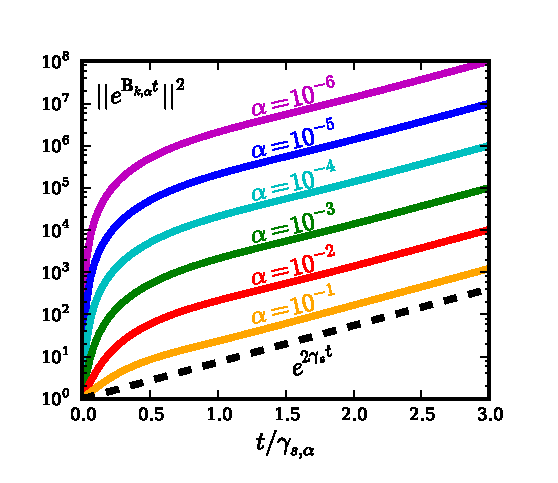
\includegraphics[width=0.45\textwidth]{max_en_growth}}
\caption{$E_{k,\alpha,\rm{max}}(t) = ||e^{\mathbf{B}_{k,\alpha} t}||^2$ for $k_x=0, k_y=1, \kappa=1$ for different values of the 2D adiabaticity parameter 
$\alpha$ compared to the energy growth $e^{2 \gamma_{s,\alpha,k} t}$ of the least stable eigenmode of  $\mathbf{B}_{k,\alpha}$. Also indicated for each matrix is its scalar normality measure $1-H$.
The time axis is normalized to $\gamma_{s,\alpha}$, which is different for each of the curves. This normalization makes the $e^{2 \gamma_{s,\alpha,k} t}$ line the same for all $\alpha$. 
$||e^{\mathbf{B}_{k,\alpha} t}||^2$ displays large non-exponential growth at early times that increases with decreasing $\alpha$.}
\label{max_en_growth}
\end{figure}

Non-normality manifests itself in the eigenvectors -- non-normal matrices or operators have nonorthogonal linear eigenvectors. For the HW model, each Fourier matrix $\mathbf{B}_k$ has two eigenvectors associated
with it. They are complex and take the form:

\beq
\label{lin_eigen_form}
\psi_{k,q} = \left( \begin{array}{cc} n_k \\ k_\perp \phi_k \end{array} \right)_q {\rm sin} \left( k_x x \right) e^{i k_y y + i k_z z} 
\eeq
where the subscript $q$ takes the values of $1$ and $2$, representing the two eigenvectors for each $k$. The two eigenvectors are different in that they have a different complex ratio $n_k/\phi_k$.
The two eigenvalues have different growth rates (the real part), but the same frequency, though with opposite sign.
As $\alpha, 1-H \to 0$, the two eigenvectors become less orthogonal -- more parallel or anti-parallel to one another. When the eigenvectors are nearly anti-parallel and initialized with finite amplitude,
their superposition, which constitutes the total system at $k$, may linearly evolve so that the norm of the superposition grows faster than either individual eigenvector. A paradigmatic illustration
of this may be seen in a review by Schmid~\cite{schmid2007}.

\section{The Effect of Non-Normality on Turbulence}
\label{sec_non_norm_turb}

Linear non-normality is important for the effect it has on turbulence. For one, non-normality is a necessary condition for turbulence in subcritical systems that have only conservative nonlinearities 
(e.g. advective nonlinearities). But it can also impact non-subcritical systems -- those which do have unstable linear eigenmodes (e.g. the 2D and 3D HW model). 
Since certain superpositions of the nonorthogonal linear eigenmodes can inject energy faster than the most unstable linear
eigenmode, there is the possibility that the energy injection into the turbulence is faster and at different wavenumbers than is suggested by linear eigenmode analysis. 

To illustrate this in the nonlinear HW model, we compare the fastest growing linear eigenmode growth rate $\gamma_{s,k}$ to the turbulent growth rate $\gamma_{t,k}$. 
In order to define the turbulent growth rate in general and specifically for the HW model, we employ a Fourier-decomposed energy dynamics analysis~\cite{camargo1995,friedman2012b,friedman2013}. 
First, we take Eqs.~\ref{n_eq} and~\ref{phi_eq} and substitute the following:

\beqar
\label{subs_fourier_n}
n = \sum_{k} n_k \ {\rm sin} \left( k_x x \right) e^{i k_y y + i k_z z} \\
\label{subs_fourier_phi}
\phi = \sum_{k} \phi_k \ {\rm sin} \left( k_x x \right) e^{i k_y y + i k_z z},
\eeqar
where, again, $k$ stands for $(k_x,k_y,k_z)$.
Then, we multiply Eq.~\ref{n_eq} by $n^*_{k'} \ {\rm sin} \left( k'_x x \right) e^{-i k'_y y - i k'_z z}$ and Eq.~\ref{phi_eq} by 
$-\phi^*_{k'} \ {\rm sin} \left( k'_x x \right) e^{-i k'_y y - i k'_z z}$, take the volume integral and add the two equations together. The result is

\beqar
\label{Explicit_En_eqn}
\frac{1}{2} \diff{}{t} \left( |n_k|^2 + k^2_\perp |\phi_k|^2 \right) = -i k_y \kappa \phi_k n^*_k - \xi k_z^2 |n_k - \phi_k|^2 \nonumber \\
- D k^4_\perp \left( |n_k|^2 + k^2_\perp |\phi_k|^2 \right) + \sum_{k'} T(k,k'). \quad \quad
\eeqar
Recall that the energy $E_k$ is $\frac{1}{2} \left( |n_k|^2 + k^2_\perp |\phi_k|^2 \right)$, so the left hand side is the time derivative of the energy.
The term $\sum_{k'} T(k,k')$ represents the nonlinear contribution (three-wave transfers between different $k$'s), 
which we do not write explicitly. This energy evolution equation may be written formally as

\beqar
\label{dEdt_def}
\diff{E_k}{t} = \diff{E_{l,k}}{t} + \diff{E_{nl,k}}{t}, \quad {\rm where}\\
\label{dEl_dt_def}
\diff{E_{l,k}}{t} = -i k_y \kappa \phi_k n^*_k - \xi k_z^2 |n_k - \phi_k|^2 \nonumber \\
- D k^4_\perp \left( |n_k|^2 + k^2_\perp |\phi_k|^2 \right) \\
\label{dEnl_dt_def}
 \diff{E_{nl,k}}{t} = \sum_{k'} T(k,k')
\eeqar
$\diff{E_{l,k}}{t}$ is composed of the linear terms on the RHS of Eq.~\ref{Explicit_En_eqn}, which are quadratic in the fluctuating quantities $n_k$ and $\phi_k$.
It describes the injection of energy into the fluctuations from the free energy in the equilibrium gradients plus the dissipation from collisions and hyperdiffusion/viscosity.
$\diff{E_{nl,k}}{t}$ represents $\sum_{k'} T(k,k')$ in  Eq.~\ref{Explicit_En_eqn} and comes from the nonlinear terms in Eqs.~\ref{n_eq} and~\ref{phi_eq}. 
The terms in $T(k,k')$ are triadic in the fluctuating quantities and account for the energy exchange between fluctuations with different $k$'s. 
They are also conservative when summed over all wavenumbers: $\sum_{k} \diff{E_{nl,k}}{t} = \sum_{k,k'} T(k,k') = 0$~\cite{camargo1995}.

Now, in quasi-steady state turbulence, the rate of net energy injection (or dissipation) into the fluctuations at each $k$ by the linear terms must be balanced by
the rate of energy removal (or deposition) from the nonlinear terms. Formally,

\beqar
\label{steady_state}
\gamma_{l,k} + \gamma_{nl,k} = \displaystyle\lim_{T \to \infty} \frac{1}{T} \int_0^T \frac{dE_k/dt}{2 E_k} dt = 0, \\
\label{gamma_l_def}
{\rm where}, \ \gamma_{l,k} \equiv \displaystyle\lim_{T \to \infty} \frac{1}{T} \int_0^T \frac{dE_{l,k}/dt}{2 E_k} dt \\
\label{gamma_nl_def}
 \gamma_{nl,k} \equiv \displaystyle\lim_{T \to \infty} \frac{1}{T} \int_0^T \frac{dE_{nl,k}/dt}{2 E_k} dt 
\eeqar
Thus, assuming steady or quasi-steady state turbulence $\gamma_{l,k} = - \gamma_{nl,k}$. Note that these, and all other growth rates, are defined to be time-independent (time-averaged) quantities.
At the scales of energy injection, $\gamma_{l,k}$ is positive and can be considered the turbulence analog of the linear eigenmode growth rate $\gamma_{s,k}$~\cite{friedman2012b,terry2006b}. 
In fact, $\gamma_{l,k} = \gamma_{s,k}$ if $n_k/\phi_k$ calculated from the nonlinear simulation is constant in time and equal to $n_k/\phi_k$ calculated from the fastest growing eigenmode at $k$. 
In general, though, these ratios are not the same because the turbulence at $k$ is composed of some linear combination of the \emph{two} eigenmodes.

\begin{table}
\begin{tabular}{|c|p {0.102\textwidth}|p {0.26\textwidth}|}
\hline
Symbol & Description & \qquad \qquad \quad Formula \\ \hline
$\gamma_s$ & Eigenmode growth rate & \qquad max(Re\{ eig( $\mathbf{B}_k$ )\})\\ \hline
$\gamma_l = \gamma_t$ & Turbulent growth rate & \quad $\displaystyle\lim_{T \to \infty} \frac{1}{T} \int_0^T \frac{dE_{l,k}/dt}{2 E_k} dt $\\ \hline
$\gamma_{nl}$ & Nonlinear growth rate & \quad $\displaystyle\lim_{T \to \infty} \frac{1}{T} \int_0^T \frac{dE_{nl,k}/dt}{2 E_k} dt = - \gamma_{l}$\\ \hline
$\gamma_{{\rm nm}}$ & Non-modal growth rate & \ $\frac{1}{4 \tau_{nl,k}} \ {\rm{Log}} \left[ {\rm{tr}} \{ e^{\mathbf{B}_k \tau_{nl,k}} e^{\mathbf{B}^{\dagger} \tau_{nl,k}} \} \right] $ \\ \hline
$\gamma_{\omega}$ & $\omega$ non-modal growth rate & \ $\frac{\omega_{s,k}}{4} \ {\rm{Log}} \left[ {\rm{tr}} \{ e^{\mathbf{B}_k \omega_{s,k}^{-1}} e^{\mathbf{B}^{\dagger} \omega_{s,k}^{-1}} \} \right]$\\ \hline
$\gamma_{\gamma}$ & $\gamma$ non-modal growth rate & \ $\frac{\gamma_{s,k}}{4} \ {\rm{Log}} \left[ {\rm{tr}} \{ e^{\mathbf{B}_k \gamma_{s,k}^{-1}} e^{\mathbf{B}^{\dagger} \gamma_{s,k}^{-1}} \} \right]$\\ \hline
\end{tabular}
\caption{Growth rate symbol descriptions and formulas}
\label{gamma_table}
\end{table}

In order to clarify that $\gamma_{l,k}$ is calculated from the quasi-steady-state portion of the nonlinear simulation, we define $\gamma_{t,k} \equiv \gamma_{l,k}$, and we call $\gamma_{t,k}$ the turbulent growth rate.
$\gamma_{t,k}$ is a useful and informative quantity. 
Note that in Eq.~\ref{Explicit_En_eqn} all of the linear terms on the right hand side of the equation are negative, except for the first term, which can have either sign. 
This term is proportional to the cross-field particle flux $\Gamma_x = \left< v_{E,x} n \right> \sim -i k_y \phi_k n_k$, meaning that a positive $\gamma_{t,k}$ indicates an outward particle flux
due to $k$ wavenumber flows. Particle transport, then, requires that $\gamma_{t,k} > 0$ for at least one value of $k$. Furthermore, since the nonlinearities are energetically conservative,
positivity of at least one $\gamma_{t,k}$ is necessary for the fluctuations to sustain themselves, meaning that it is a necessary condition for turbulence and transport. 
Finally, through the mixing length approximation $|\phi| \sim \frac{\gamma_{t,k}}{k_\perp^2}$, $\gamma_{t,k}$ can provide an estimate of the turbulent saturation level.

In turbulent systems with normal linear operators $\gamma_{t,k} \le \gamma_{s,k}$. This is evident if one recalls that in normal systems, the maximal
energy growth is given by the most unstable linear eigenmode. In other words, maximal growth is achieved when only the most unstable eigenmode has finite amplitude.
If the stable eigenmode has finite amplitude, it decreases the turbulent growth rate.
On the other hand, non-normal systems may grow faster when the stable eigenmodes have finite amplitude than when they have none (see Fig.~\ref{max_en_growth}). 
It is therefore possible for $\gamma_{t,k} > \gamma_{s,k}$ in non-normal systems.

For the 2D HW model, we show
$\gamma_{s,k}$ and $\gamma_{t,k}$ for two different values of $\alpha$. In Fig.~\ref{alpha1e-5_gamma_s_t}, we show these growth rate spectra for $\alpha = 10^{-5}$, for which the system is
highly non-normal, and in Fig.~\ref{alpha1_gamma_s_t} for $\alpha = 1$, for which the system is closer to being normal (see the inset of Fig.~\ref{gamma_max_vs_alpha}). All calculations in this section use $\kappa=1$. 
In the highly non-normal case, the turbulent growth rate is very similar to the eigenmode growth rate for most values of $k_x,k_y$, but about 6 times higher where the spectrum peaks. For the more normal
case, in contrast, $\gamma_{t,k}$ is generally lower than $\gamma_{s,k}$, with the peak at nearly a factor of 2 less, with the peaks being at slightly different values of $k_y$.
\begin{figure}
\centerline{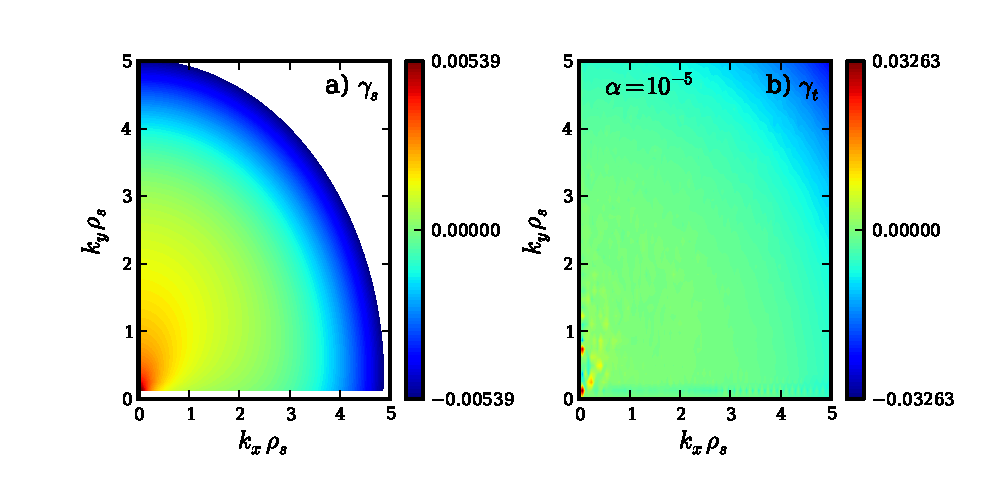
\includegraphics[width=0.52\textwidth]{alpha1e-5_gamma_s_t}}
\caption{{\bf a)} The eigenmode growth rate spectrum $\gamma_{s,k}$ and {\bf b)} the turbulent growth rate spectrum $\gamma_{t,k}$ for $\alpha = 10^{-5}, \kappa=1$.}
\label{alpha1e-5_gamma_s_t}
\end{figure}

Since the peak growth rates are the most important when considering whether a system can sustain turbulence, we show the peak values for $\gamma_{s,k}$ and $\gamma_{t,k}$ in Fig.~\ref{gamma_max_vs_alpha} as a function of $\alpha$. 
The peak values always occur in $k$-space at the lowest $k_x$ available to our system, corresponding to half of a period of a sine wave. The value of $k_y$ that gives the highest growth rate migrates upward as $\alpha$ increases,
as is clear from Figs.~\ref{alpha1e-5_gamma_s_t} and~\ref{alpha1_gamma_s_t}. Henceforth, we discuss only the peak growth rates.

As expected, when $\alpha$ is small ($\lesssim 10^{-3}$), $\gamma_{t} > \gamma_{s}$, with
$\gamma_{t} \gg \gamma_{s}$ as $\alpha \to 0$. Additionally, when $\alpha$ becomes larger and the system becomes more normal ($\gtrsim 10^{-1}$), $\gamma_{t} < \gamma_{s}$.
For both the normal and highly non-normal limits of the 2D HW model, $\gamma_{s}$ does a poor job of predicting $\gamma_{t}$ because $\gamma_{s}$ neglects the stable branch of the
dispersion relation -- the damped eigenmode~\cite{makwana2011}. 
Additionally, in the moderate non-normality region where $\gamma_{s}$ does match $\gamma_{t}$ well, it is misleading to think of the system as being composed of only the unstable eigenmode. 
The damped mode simply has both damping and transient growth effects depending on its relative magnitude at a particular time. These effects nearly cancel out on average when $\gamma_{t} \approx \gamma_{s}$.

\begin{figure}
\centerline{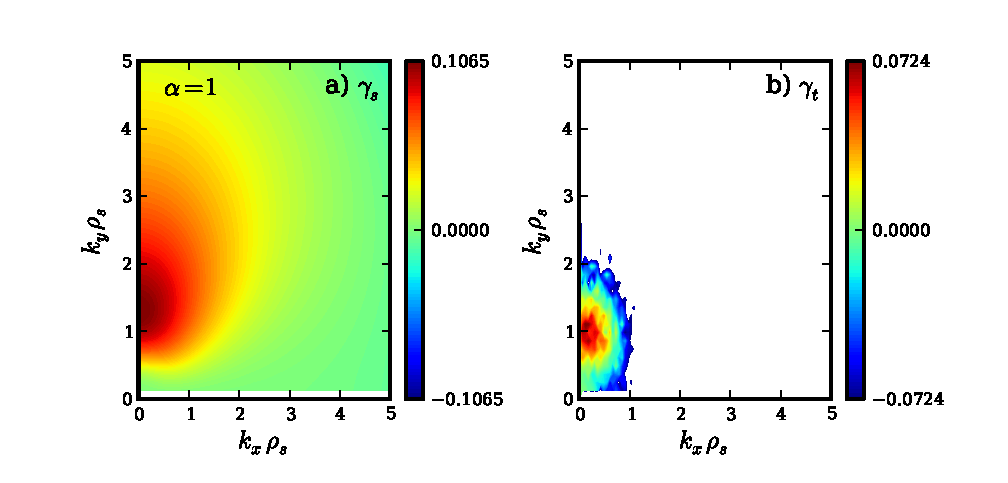
\includegraphics[width=0.52\textwidth]{alpha1_gamma_s_t}}
\caption{{\bf a)} The eigenmode growth rate spectrum $\gamma_{s,k}$ and {\bf b)} the turbulent growth rate spectrum $\gamma_{t,k}$ for $\alpha = 1, \kappa=1$.}
\label{alpha1_gamma_s_t}
\end{figure}

The importance of the stable eigenmode branch~\cite{baver2002} (or branches) has started to gain acceptance in the plasma community, although it has generally been used in normal
or nearly normal systems to explain turbulent saturation~\cite{terry2006b,hatch2011,makwana2011} ($\gamma_{t} < \gamma_{s}$). 
The case of highly non-normal turbulence and the associated increased turbulent excitation hasn't been understood as well. 
In fact, simulation and analysis of the 3D HW model (and extended models) is an area in which others have seen the effects of strong non-normal transient growth
but have not connected them to the nonorthogonal eigenmode transient growth theory~\cite{biskamp1995,drake1995,scott2002,scott2005,umansky2009,friedman2012b}.

As Biaskamp and Zeiler~\cite{biskamp1995} discovered, the 3D HW model nonlinear simulation has a fascinating property -- 
the turbulent energy injection is positive at $k_z = 0$ despite the fact that there can be no unstable linear eigenmodes at $k_z=0$.
In fact, for high enough values of $\xi$ ($\xi \ge 10^2$), more energy is injected at $k_z = 0$ than at finite $k_z$ (see Fig.~\ref{gamma_max_vs_xi} below for more details).
We show this in Fig.~\ref{gamma_max_vs_kz} using the eigenmode $\gamma_{s,k}$ and turbulent $\gamma_{t,k}$ growth rates, plotting them as a function of $k_z$.
The long-stated cause of this $k_z=0$ energy injection is a nonlinear instability~\cite{biskamp1995,drake1995}. 
The nonlinear instability works as follows: magnetic-field-aligned ($k_z=0$) convective cells transport density across the equilibrium density gradient, setting up $k_z=0$ density structures. 
These structures are unstable to drift waves, which grow as a secondary instability.
The secondary drift waves, which have finite $k_z$, nonlinearly couple to one another and reinforce the original convective cells (or generate new ones), leading to self-sustainment.

Although the instability is a nonlinear instability, the first part of the mechanism -- the transport of background density by the convective cells -- is a linear one. This process occurs at $k_z=0$
for which the adiabaticity parameter iz zero ($\alpha = k_z^2 \xi = 0$) meaning the linear matrix operator is highly non-normal and subject to transient growth.
So non-normal effects play a role in the 3D HW system for all $\xi$ due to the presence of $k_z=0$ structures.

\begin{figure}
\centerline{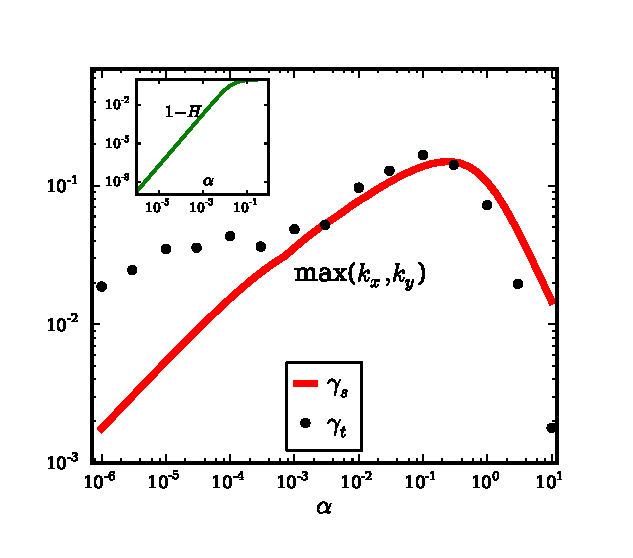
\includegraphics[width=0.4\textwidth]{gamma_max_nn}}
\caption{The eigenmode $\gamma_{s}$ and turbulent $\gamma_{t}$ growth rates as a function of $\alpha$, which controls the normality of the linear operator. All growth rates are peaks in $k_x-k_y$ space.
The insert shows the scalar normality measure $1-H$ as a function of $\alpha$ for the matrices $\mathbf{B}_k$ that give the $\gamma_{s}$ curve.}
\label{gamma_max_vs_alpha}
\end{figure}

\begin{figure}
\centerline{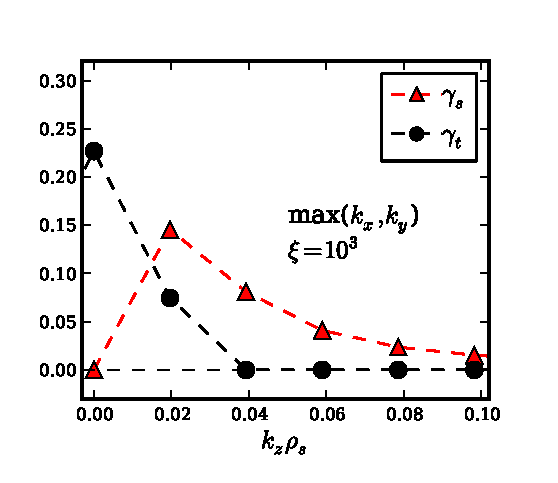
\includegraphics[width=0.4\textwidth]{gamma_max_vs_kz}}
\caption{The growth rates of the fastest growing eigenmode $\gamma_{s,k}$ and the of the turbulence $\gamma_{t,k}$ as a function of $k_z$ for the 3D HW model at $\xi = 10^3$. The most remarkable feature is
that the turbulent growth rate peaks at $k_z=0$ despite the stability of all linear eigenmodes at $k_z=0$.}
\label{gamma_max_vs_kz}
\end{figure}

\section{Non-Modal Linear Procedure To Calculate Turbulent Growth Rate}
\label{sec_nm_procedure}

In this section, we outline a procedure that uses quick and simple methods to approximate the turbulent growth rate spectrum $\gamma_{t,k}$. To do this, first recall that $\gamma_{t,k}$ is calculated
from only linear terms in the original model equations (Eqs.~\ref{n_eq} and~\ref{phi_eq}). The exact form of the nonlinearities do not enter the calculation of $\gamma_{t,k}$. Rather, the nonlinearities
simply influence the quantities $n_k$ and $\phi_k$ that are used to calculate $\gamma_{t,k}$. Furthermore, $\gamma_{t,k}$ is a statistical (time-averaged) quantity, and therefore, it is not
necessary to know its instantaneous value, or likewise, the instantaneous values of $n_k$ and $\phi_k$. In fact, the only quantity that affects $\gamma_{t,k}$ is the average complex ratio $n_k/\phi_k$.
Thus, it is feasible that $\gamma_{t,k}$ may be approximated without numerical simulation.

Our method of approximation involves modeling the nonlinearities as instantaneous randomizing forces that act periodically.
In this regard, note that the advective nonlinearity terms in Eqs.~\ref{n_eq} and~\ref{phi_eq} have a certain time scale associated with them: $\tau_{nl}^{-1} \sim v_E k_\perp$.
This nonlinear time scale is generally associated with the eddy turnover or decorrelation time. Our heuristic model of the nonlinearities is then one
in which they randomize the complex ratio $n_k/\phi_k$ once every $\tau_{nl}$.
This model equivalently describes a system in which 1) the turbulence begins as a random state, 
2) evolves linearly for a time $\tau_{nl}$, and 3) randomizes again -- due to nonlinear energy transfer -- at which point the step 2 is repeated and so on.

What makes this model truly appealing is its simplicity. In fact, we can use it to \emph{analytically} calculate an effective growth rate. It requires no numerical simulation.
To see this, recall that the linear time evolution of the energy from an initial condition is

\beq
\label{E_t_from_u0}
E_k(t) = ||e^{\mathbf{B}_k t} u(0)||^2 = e^{\mathbf{B}_k t} u(0) u^{\dagger}(0) e^{\mathbf{B}_k^{\dagger}t}.
\eeq
where $e^{\mathbf{B}_k^{\dagger}t}$ is shorthand for $\left( e^{\mathbf{B}_k t} \right)^{\dagger}$.
Since $\gamma_{t,k}$ is a time-averaged quantity and the nonlinear model randomizes the system periodically, we can use an ensemble of initial conditions ($u(0)$'s that are random normalized vectors with uncorrelated components),
and take two averages (over $t=0$ to $t = \tau_{nl}$ and over the ensemble) in place of the single time average that is generally used to calculate $\gamma_{t,k}$. The two averages commute, but for simplicity, 
we look at each average separately and then put them together.

For the ensemble average, Camargo et al.~\cite{camargo1998,friedman2014} showed that the ensemble average of the energy evolution in Eq.~\ref{E_t_from_u0} could be simplified as,

\beq
\label{E_t_ensemble_avg}
\left< E_k(t) \right>_{{\rm{ens}}} = \frac{1}{2} {\rm{tr}} \{ e^{\mathbf{B}_k t} e^{\mathbf{B}_k^{\dagger}t} \},
\eeq
where we have initialized $||u(0)||^2 = 1$ for convenience.

Second, the short-time averaged growth rate from $t=0$ to $t = \tau_{nl}$ is simplified as,

\beq
\label{gamma_nm_calc}
\frac{1}{\tau_{nl,k}} \int_0^{\tau_{nl,k}} \frac{\pdiff{E_k(t)}{t}}{2 E_k(t)} dt = \frac{1}{2 \tau_{nl,k}} \ {\rm{Log}} \left[ \frac{E_k(\tau_{nl,k})}{E_k(0)}\right].
\eeq

Now, putting these commuting averages together, and again setting $E_k(0) = 1$ for normalization, we arrive at the non-modal growth rate:

\beq
\label{gamma_nm}
\gamma_{{\rm{nm}},k} = \frac{1}{4 \tau_{nl,k}} \ {\rm{Log}} \left[ {\rm{tr}} \{ e^{\mathbf{B}_k \tau_{nl,k}} e^{\mathbf{B}^{\dagger} \tau_{nl,k}} \} \right].
\eeq
Note that the factor of $\frac{1}{4}$ is particular to two-field systems. Namely, the factor of $\frac{1}{2}$ coming from Eq.~\ref{E_t_ensemble_avg} is a consequence of $\mathbf{B}_k$ being a rank-$2$ matrix.

\begin{figure}
\centerline{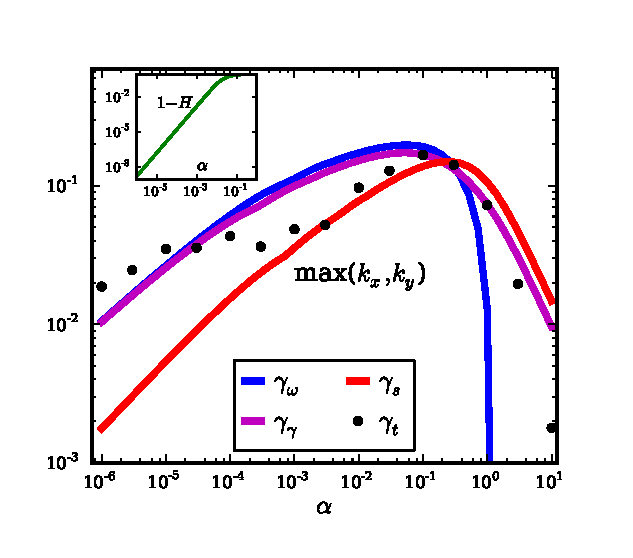
\includegraphics[width=0.4\textwidth]{gamma_max_with_nm_nn}}
\caption{Comparison of the non-modal growth rates $\gamma_{\omega,k}$ and $\gamma_{\gamma,k}$ to the eigenmode $\gamma_{s}$ and turbulent $\gamma_{t}$ growth rates as a function of $\alpha$ for the 2D HW model. 
All growth rates are peaks in $k_x-k_y$ space.}
\label{gamma_max_with_nm}
\end{figure}

Finally, in order to obtain a simple and quick prediction of $\gamma_{{\rm{nm}},k}$, we must estimate $\tau_{nl,k}$ without having to calculate it directly from a turbulent simulation. 
We thus invoke the conjecture of \emph{critical balance}, which posits that the nonlinear time scale equals a characteristic linear time scale at all spatial scales~\cite{schekochihin2012}. 
There are a few possible linear time scales in the HW problem to use for $\tau_{nl,k}$ 
including the inverse linear eigenmode frequency and growth rates as well as certain times associated with transient growth curves.

We choose to test two of these linear time scales -- the inverse linear eigenmode frequency $\omega_{s,k}^{-1}$ and the inverse least stable eigenmode growth rate $\gamma_{s,k}^{-1}$, corresponding to the imaginary and real parts
of the dominant eigenvalue of the linear matrix operator $\mathbf{B}_k$.
The reason for using the least stable eigenmode growth rate rather than the most stable growth rate is that the least stable one should contribute more to the nonlinearity at long time after the randomization step.
As for the eigenmode frequency, recall that the imaginary part of the linear eigenvalues is the same for both eigenvalues of $\mathbf{B}_k$, so there is no question of which eigenfrequency to use. 
We thus arrive at our final definition for the non-modal growth rates:

\beqar
\label{gamma_omega_def}
\gamma_{\omega,k} = \frac{\omega_{s,k}}{4} \ {\rm{Log}} \left[ {\rm{tr}} \{ e^{\mathbf{B}_k \omega_{s,k}^{-1}} e^{\mathbf{B}^{\dagger} \omega_{s,k}^{-1}} \} \right] \\
\label{gamma_gamma_def}
\gamma_{\gamma,k} = \frac{\gamma_{s,k}}{4} \ {\rm{Log}} \left[ {\rm{tr}} \{ e^{\mathbf{B}_k \gamma_{s,k}^{-1}} e^{\mathbf{B}^{\dagger} \gamma_{s,k}^{-1}} \} \right].
\eeqar
Eqs.~\ref{gamma_omega_def} and~\ref{gamma_gamma_def} are analytic expressions that require no numerical simulation. 
Furthermore, since the $k$'s have been decoupled by the model, one does not have to perform calculations for many values of $k$, making all calculations extremely fast compared to nonlinear simulations.

\begin{figure}
\centerline{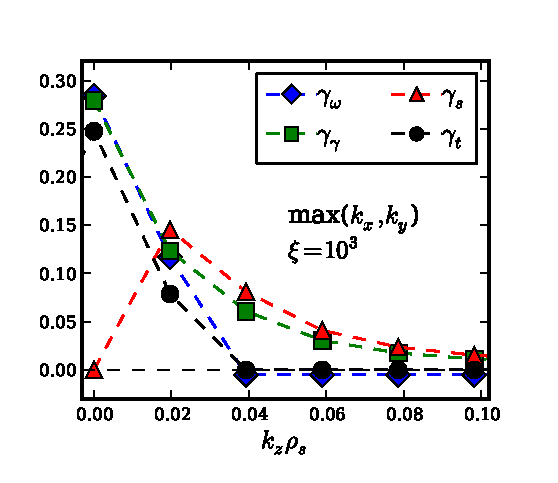
\includegraphics[width=0.4\textwidth]{gamma_max_vs_kz_with_nm}}
\caption{Comparison of the non-modal growth rates $\gamma_{\omega,k}$ and $\gamma_{\gamma,k}$ to the growth rates of the fastest growing eigenmode $\gamma_{s,k}$ 
and the of the turbulence $\gamma_{t,k}$ as a function of $k_z$ for the 3D HW model with $\xi = 10^3$. The non-modal growth rates correctly predict the growth rate dominance of the $k_z=0$ mode
despite the $k_z=0$ eigenmode stability.}
\label{gamma_max_vs_kz_with_nm}
\end{figure}

We test the model against the full direct numerical simulations (DNS) by comparing $\gamma_{\omega,k} \rm{and} \ \gamma_{\gamma,k}$ to $\gamma_{t,k}$. 
As seen in Fig.~\ref{gamma_max_with_nm}, the peak non-modal growth rate predictions for 2D HW turbulence generally agree within a factor of 2 with the turbulent growth rate. For $\alpha \le 10^{-4}$,
in which the system is fairly non-normal, $\gamma_{\omega,k} \rm{and} \ \gamma_{\gamma,k}$ predict $\gamma_{t,k}$ quite accurately, especially compared to the eigenmode prediction. 
This limit, of course, is important in subcritical systems, making the non-modal growth rates quite useful.
As the system becomes more normal, $\gamma_{t,k}$ diverges from $\gamma_{\omega,k} \rm{and} \ \gamma_{\gamma,k}$, with $\gamma_{\gamma,k}$ doing a better job than $\gamma_{\omega,k}$.

Next, we do the same comparison for the 3D HW model as we did for the 2D HW model. However, there is one additional subtlety when considering the 3D model. In the 3D model, for $k_z=0$, the least stable linear
eigenmode is approximately zero ($\omega_{s,k_z=0} = 0, \gamma_{s,k_z=0} \approx 0$), so $\gamma_{\omega,k_z=0}$ is not well defined (see Eq.~\ref{gamma_omega_def}), and $|\gamma_{s,k_z=0}^{-1}|$ is much too large to
represent a meaningful time scale. 
Thus, we use $\omega_{s,k_z=0.02}$ -- where $k_z=0.02$ is the lowest finite value of $k_z$ available to our system -- in place of
$\omega_{s,k_z=0}$ in the calculation of $\gamma_{\omega,k_z=0}$ (and similarly for $\gamma_{s,k_z=0}$). 
We contend that the nonlinear instability, which most strongly couples $k_z=0$ and $k_z=0.02$ modes, has its time scale set
by the drift waves, not the convective cells, making $\omega_{s,k_z=0.02}^{-1}$ and $\gamma_{s,k_z=0.02}^{-1}$ good proxies for $\tau_{nl,k_z=0}$~\cite{friedman2014}. 

Despite these complications at $k_z=0$,  $\gamma_{\omega,k} \rm{and} \ \gamma_{\gamma,k}$ approximate $\gamma_{t,k}$ remarkably well, even when the linear matrix is only moderately ($1-H \approx 10^{-1}$) non-normal
(see Figs.~\ref{gamma_max_vs_kz_with_nm} and~\ref{gamma_max_vs_xi}). And again, $\gamma_{\gamma,k}$ is better at higher $\xi$ than $\gamma_{\omega,k}$, though here $\gamma_{\omega,k}$ gives the better prediction
at some intermediate values of $\xi$. Most importantly, however, they both correctly predict that $\gamma_{t,k_z=0} > 0$.
Therefore, non-modal calculations explain why the 3D HW model can be dominated by the nonlinear instability rather than a linear drift wave instability. 
Simply put, the transient growth rate may be largest at $k_z=0$ so the nonlinear instability is energetically favored over the primary drift wave instability.

\begin{figure}
\centerline{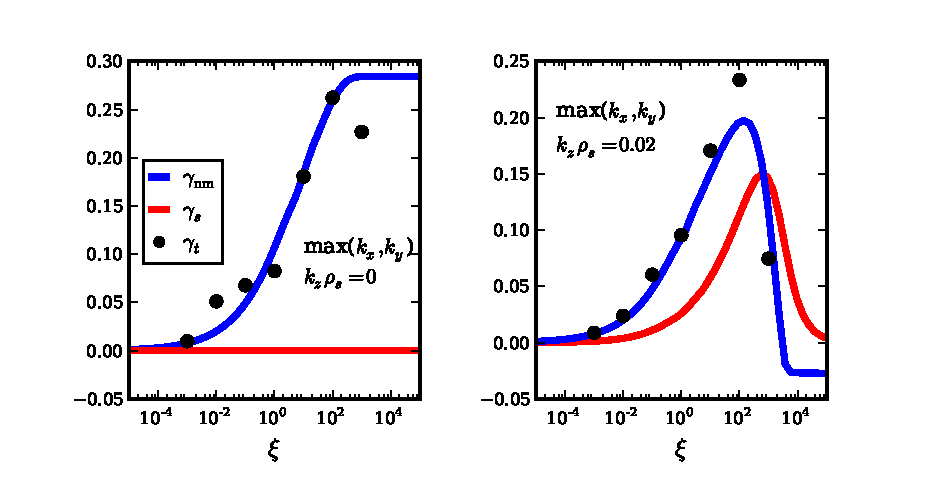
\includegraphics[width=0.52\textwidth]{gamma_max_vs_xi}}
\caption{Comparison of the peak non-modal growth rates $\gamma_{\omega,k} \ $ and $\gamma_{\gamma,k}$ to that of the fastest growing eigenmode $\gamma_{s,k}$ 
and the turbulence $\gamma_{t,k}$ as a function of $\xi$ for the 3D HW model at {\bf a)} $k_z \rho_s = 0$ and {\bf b)} $k_z \rho_s \approx 0.02$. }
\label{gamma_max_vs_xi}
\end{figure}

\section{Prediction of Control Parameter for Subcritical Turbulent Onset}
\label{sec_subcrit_prediction}

In both hydrodynamic and plasma systems, it is important to be able to predict for a given set of parameters whether the system will be turbulent or not.
Ideally, one would like to find the point, line, or manifold in parameter space that divides turbulent and laminar solutions.
In many hydrodynamic systems with sheared flow, there is generally a single control parameter -- the Reynold's number $Re$~\cite{drazin1981}. For high enough $Re$ such systems
can be turbulent, but for low $Re$ they are always laminar.
Normal systems will undergo a bifurcation from a laminar to non-laminar state when the control parameters are such that at least one of the linear eigenmodes is unstable~\cite{grossmann2000}.
In general, this is not true for non-normal systems. In many non-normal systems, turbulence can be sustained when all linear eigenmodes are stable -- the case of subcritical turbulence. 

Subcritical systems fall into two categories: those that have stable eigenmodes for all values of the control parameter, and those that have unstable eigenmodes
when the control parameter becomes large (or small) enough. We illustrate these two categories with a diagram in Fig.~\ref{subcritical_diagram}. 
The upper curve represents the first kind of subcritical system in which no unstable eigenmodes exist for any value of the control parameter $R$. In this
case, there is some transitional value of $R$, labeled $R_g$, below
which turbulence cannot occur. When a perturbation with amplitude
($A$) above the line occurs in the system due to external input or noise, 
turbulence will be excited. Perturbations with amplitude below the line will decay away. The higher the value of $R$, the smaller the perturbation needs to be to excite turbulence.
Experimental evidence and theoretical arguments show this curve should have a $(R-R_g)^{-\lambda}$ dependence (for asymptotically large $R$), with $\lambda \sim 1$~\cite{waleffe1995b,grossmann2000,hof2003}.
A paradigmatic example of this kind of system is Hagen-Poisuille pipe flow -- flow in a cylindrical pipe with a parabolic flow profile -- for which $R_g \approx 2000$.

The lower curve represents the second kind of subcritical system. Above a critical value of the control parameter $R_c$, the system is linearly unstable. But, for $R_g < R < R_c$, the system is
unstable to finite amplitude perturbations, or ``nonlinearly'' unstable. A paradigmatic example of this is Poissuille channel flow -- the rectangular analog of pipe flow -- for which
$R_c = 5772$ and $R_g \approx 1000$~\cite{grossmann2000}. Most subcritical magnetically-confined plasma systems fall into this category. It is perhaps easy to be fooled into believing that the turbulence
in such systems is due to eigenmode instability even though it may not be. 
In either case, one of the most important predictions is the minimum turbulent control parameter $R_g$, which is sometimes called the ``transitional'' value of the control parameter. Given that this problem is many decades old
and still unsolved, it is a tall order to predict $R_g$ without nonlinear simulations. We nevertheless make an attempt using our procedure for calculating $\gamma_{\rm{nm}}$.

The HW model in an unsheared magnetic slab is not subcritical in either the 2D or 3D cases, as implied by Figs.~\ref{gamma_max_vs_alpha} and~\ref{gamma_max_vs_kz}. It is subcritical in a highly sheared
magnetic field~\cite{drake1995}, but the eigenmodes of the linear operator in that case are not sinusoidal, making our non-modal analysis more difficult. 
Biskamp et al.~\cite{biskamp1995}, however, artificially modified the
3D HW model to remove the linear drive by taking the $z$-average of the $\kappa \pdiff{\phi}{y}$ term in Eq.~\ref{n_eq}, effectively eliminating the $k_z \ne 0$ drive. This leaves only the $k_z = 0$
component of the drive term. Since the $k_z = 0$ eigenmodes are stable but $k_z = 0$ structures can access the free energy (positive $\gamma_t$ in Fig.~\ref{gamma_max_vs_kz}), this system is subject
to subcritical turbulence.

\begin{figure}
\centerline{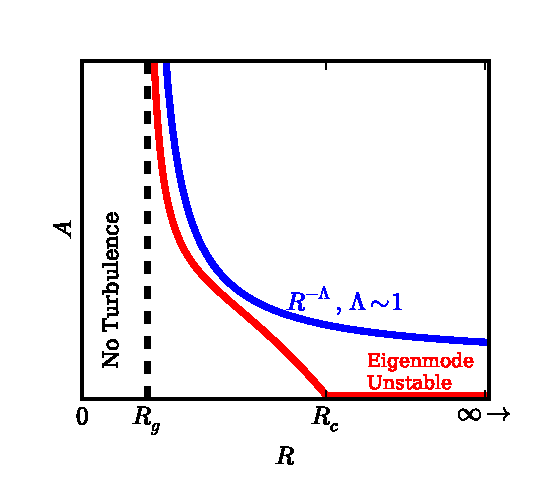
\includegraphics[width=0.4\textwidth]{subcritical_diagram}}
\caption{Diagram of a control parameter $R$ versus perturbation amplitude $A$ for two subcritical systems. The first curve (top blue one with $(R-R_g)^{-\lambda}$ label) represents a system with no
eigenmode instability for any $R$, but which is stable to finite amplitude perturbations for $R > R_g$. 
The second (bottom red one with label of ``Eigenmode Unstable'') represents a system with a linear eigenmode instability for $R \ge R_c$, and finite amplitude
instability for $R_g < R < R_c$.}
\label{subcritical_diagram}
\end{figure}

We show that the modified 3D HW system is subcritical in Fig.~\ref{crit_amp_dependence}. In Fig.~\ref{crit_amp_dependence} a), we plot the energy versus time for fluctuations that are initialized with the same functional form, but with
different amplitudes.
The fluctuations initialized with high enough amplitude lead to turbulence. 
Otherwise, the fluctuations grow transiently, but do not reach high enough amplitude for the nonlinearities to bootstrap the process, so they decay away. 
This finite amplitude turbulence threshold, as described above, is a key indicator of subcritical turbulence.

In Fig.~\ref{crit_amp_dependence} b), we show the amplitude threshold curve -- like that of Fig.~\ref{subcritical_diagram}. Each point represents the minimum amplitude that is needed for the simulation to eventually become
turbulent. We fit the points to a function of the form $A = a (\kappa - \kappa_g)^{- \lambda}$, 
where $A$ is the lowest initial energy amplitude that leads to turbulence for each value of $\kappa$. The least-squares fitting provides optimal values for the parameters $a, \kappa_g, \rm{and} \ \lambda$. 
As in the case of shear flows, $\lambda \sim 1$. Note that this power law exponent shouldn't be taken too seriously because we have not used ``optimal'' initial perturbations to get the points~\cite{cossu2005}. 
In any case, this is not our main concern; we are simply demonstrating that this modified 3D HW model is subcritical.

\begin{figure}
\centerline{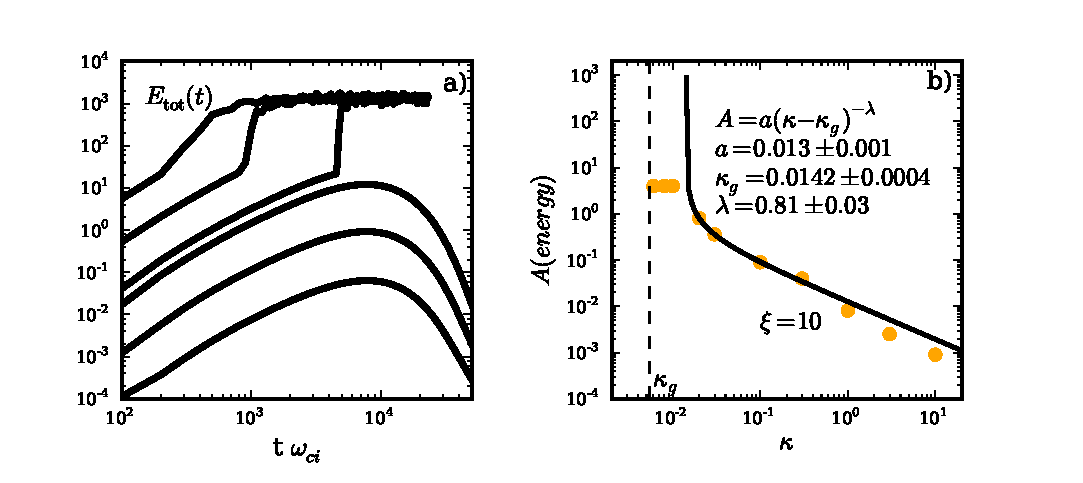
\includegraphics[width=0.52\textwidth]{crit_amp_dependence}}
\caption{{\bf a)} Total energy evolution of fluctuations of the modified 3D HW model with $\xi=10$ and $\kappa=1$ where the initial perturbations are set to different amplitudes. 
All initial perturbations are initialized randomly in the $y$ and $z$ directions and with a Gaussian in the $x$ direction. 
There is a critical initial amplitude threshold above which turbulence develops and maintains itself and below which turbulence never develops and the fluctuations decay away. 
{\bf b)} The amplitude threshold as a function of $\kappa$ for $\xi=10$. The points are obtained from nonlinear simulations like those in part a) with each point indicating the minimum amplitude needed for the simulation
to become turbulent. The line is a fit to the points with the functional form $a (\kappa-\kappa_g)^{- \lambda}$.
We set the diffusion and viscosity coefficient $D$ to $0.5$ in these figures so that the decay occurs on a short enough time scale to be able to see the results.}
\label{crit_amp_dependence}
\end{figure}

For this subcritical system, we predict the transitional dividing line $\kappa_g(\xi)$ that separates the parameter space into turbulent and laminar sections. In the turbulent section, 
fluctuations initialized with high enough amplitude can drive turbulence. In the laminar section, fluctuations will all eventually decay no matter how large they are initialized. 
In the turbulent section, it is not necessarily the case that the system will look turbulent in the usual sense, at least not strongly turbulent.
So more accurately, in the turbulent section, the system will undergo some sort of bifurcation that brings with it sustained finite transport.

We show the answer that we obtain from nonlinear simulations along with our non-modal predictions in Fig.~\ref{subcrit_param_space}. To obtain $\kappa_g(\xi)$ from the nonlinear simulations,
rather than mapping out curves like those in Fig.~\ref{crit_amp_dependence} b), we simply start all simulations with a large initial amplitude ($A = 10^4$) and vary $\kappa$ until we find the minimum $\kappa$ that
permits a sustained positive value of the turbulent growth rate $\gamma_{t,k}$.
Similarly, we find the lines (with a root-finding routine) in $\xi-\kappa$ space at which $\gamma_{\omega} = 0$ and $\gamma_{\gamma} = 0$, using the lowest permissible values of $k_x$ and $k_y$, which maximize the growth rates. 
We plot these lines in Fig.~\ref{subcrit_param_space}.

\begin{figure}
\centerline{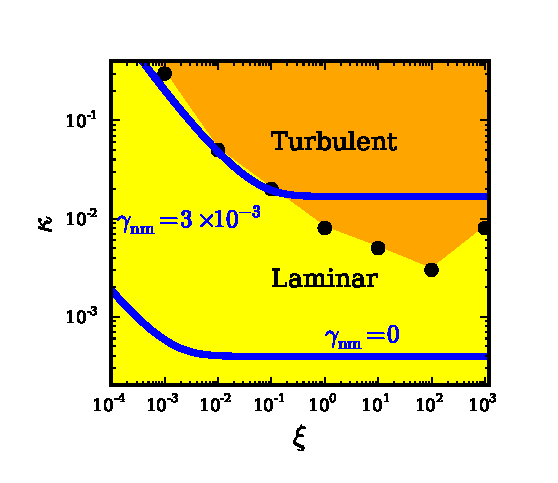
\includegraphics[width=0.4\textwidth]{subcrit_param_space}}
\caption{The non-modal curves $\gamma_{\omega}(\kappa,\xi) = 0$ and $\gamma_{\gamma}(\kappa,\xi) = 0$ predict the transitional value of $\kappa(\xi)$ for the subcritical 3D HW model. The points represent the
transitional values of $\kappa(\xi)$ based on full nonlinear simulations.}
\label{subcrit_param_space}
\end{figure}

Clearly, our non-modal procedure with our particular choice of linear time scales does not provide even an order-of-magnitude accurate prediction of $\kappa_g$ for all values of $\xi$.
Nevertheless, the non-modal predictions display some qualitative agreement with the DNS results in that the non-modal predictions trend fairly accurately with $\xi$. 
And they do provide a prediction to the transition density gradient $\kappa_g$ in contrast to the eigenmode growth rates, which are always negative in this system and thus do not predict turbulence for any $\kappa$.
So, there is some value in the non-modal predictions, especially in light of the fact that it took over $10^5$ computer hours to calculate the $\kappa_g$ line using DNS and only seconds using the non-modal procedure.
Furthermore, it is likely that more sophisticated models for the nonlinearities will improve the predictions in the future.

\section{Conclusion}

When the nonlinear terms in the model equations are energetically conservative, as they are in the HW model, the linear terms must on average inject energy into at least one wavenumber to sustain turbulent fluctuations.
This is manifest in the positivity of the maximum turbulent growth rate, which is defined in terms of only the linear terms in the energetic model equations. Thus, an estimation of the turbulent growth rate provides vital
information into the nature of the system. Furthermore, such an estimate almost surely requires non-modal techniques when the system is non-normal. 

Our method for analytically estimating this growth rate involves using a type of closure, which means modeling the effect that the nonlinearities have
on the time-averaged complex ratio of the Fourier-decomposed state variables. 
We present one specific phenomenological closure, in which the nonlinearities instantaneously randomize the state variables once every eddy turnover time, between
which, the linear terms deterministically evolve them. We then estimate the eddy turnover time as the inverse linear eigenmode frequency or growth rate.

While our nonlinear closure model is successful in some instances, such as the highly non-normal limit in the 2D HW model and in the 3D HW model when the gradient scale length factor $\kappa$ is large, it is relatively unsuccessful
in others, especially when the system is not highly non-normal. This prevents an accurate prediction of the transitional value $\kappa_g$ that marks where the system first becomes turbulent.
Perhaps in the future, more advanced closure techniques will allow for better approximation of the turbulent growth rate.

\begin{acknowledgments}
This work was supported by the National Science Foundation (Grant PHY-1202007)
\end{acknowledgments}

%%%%%%%%%%%%%%%%%%%%%%%%%%%%%%%%%%%%%%%%%%%%%%%%%%%%%%%%%%%%%%%%%%%%%%%%%%%

%\bibliographystyle{phaip}
\bibliography{refs}

\end{document}
